\documentclass[../main.tex]{subfiles}
\graphicspath{{\subfix{../images/}}}

\begin{document}

\chapter{State of the Art}

\section{The \davinci Surgical System}
Since the FDA approval recieved by Intuitive Surgical Inc. (Sunnyvale, CA, USA) in 2000, the surgical robotics market has been dominated by the \davinci surgical system and its multiple evolutions (\textit{daVinci X}, \textit{daVinci Xi}, \textit{daVinci Si} and most recently the \textit{daVinci SP}). In 2021 there were more than 6,500 \textit{daVinci} surgical systems installed in 67 countries, and more than 55000 surgeons worldwide have been trained on the use ofit \cite{Intuitive2021}. The numerous advantages in safety, non-invasiveness, precision and dexterity were the key factors that made this technology so disruptive, as well as the role that this surgical robot was designed to undertake in the \ac{or}: it is, as a matter of fact, a tool for the surgeon to exploit to enhance his performance, and not a replacement for the surgeon himself.

Three distinct componets make up a \textit{daVinci} surgical system:
\begin{itemize}
   \item The \textbf{Surgeon Console} accomodates the practictioner and acts as the primary interface between him and the robot. Seated at the console the surgeon grips the \mtms to control the motion of the robot arms, sees in 3D the surgical scene by looking into the \ac{hrsv} and presses foot-switches to change specific settings (Figure \ref{fig:davincisystem} left and Figure \ref{fig:surgeonconsolepanel}).
    \item The \textbf{Patient Cart} is positioned next to the patient, and it mounts the \psms and the \ecm. The \psms are the robot arms that are used to manipulate the surgical instruments, while the \ecm is used to control the stereo endoscope camera (Figure \ref{fig:davincisystem} right and Figure \ref{fig:patientcartpanel})
    \item The \textbf{Vision Cart} handles the communication between all the hardware components, and it is responsible for the image processing and the motion planning of the robot arms (Figure \ref{fig:davincisystem} center).
\end{itemize}

\begin{figure}
    \centering
    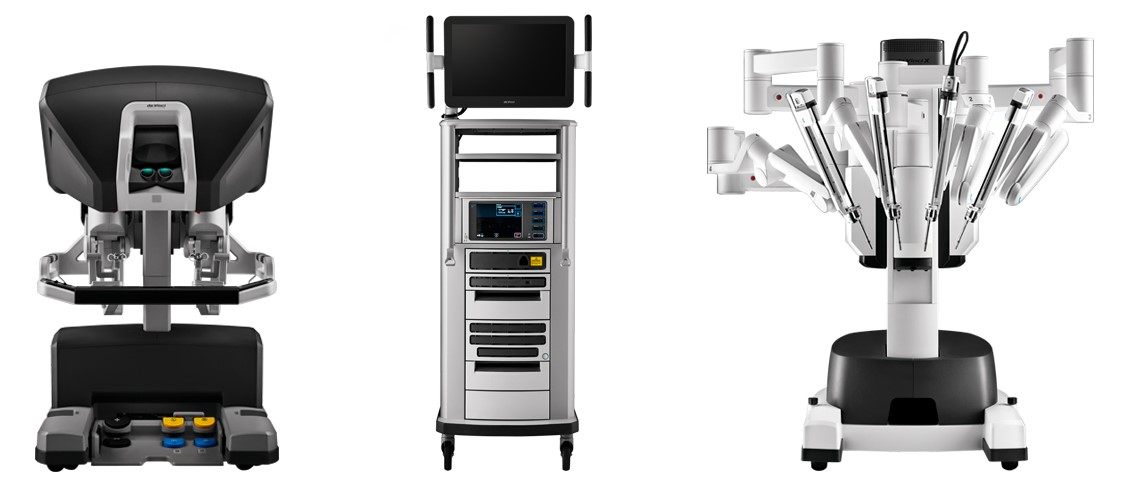
\includegraphics[width=\textwidth]{images/davinci_system.jpg}
    \caption{The macro constituents of a \davinci surgical system in the operatory room: the Surgeon Console (left), the Vision Cart (middle) and the Patient Cart (right).}
    \label{fig:davincisystem}
\end{figure}

\subsection{The Surgeon Console}
The console is the main input-output interface between the surgeon and the robotic arms. The surgeon, in fact, holds the grippers of the \mtms (one for the right hand and one for the left hand) and moves his hands, wrists and fingers. Each \mtm is a 8 degrees-of-freedom serial kinematic chain: by knowing the coordinate of each rotational joint in the chain, the position and orientation of the gripper in the cart reference frame is known through forward kinematics. A detailed kinematics analysis of the \davinci was conducted in \cite{Fontanelli2017}, and the Denavit-Hartenberg (DH) parameter for FK and IK are determined asweel. 

The pose of the \mtms grippers with respect to the console reference frame will then be used to compute the desired position of the end-effector of the \psms, and inherently the joint coordinates through an inverse kinematics algorithm.

Seated at the console, the practitioner feels immersed into the surgical scene thanks to the 3D viewing capability of the \hrsv. This pair of oculars is directly connected to the pair of cameras situated on the \ecm: the disparity between the images displayed in the left and right lenses gives the surgeon the perception of depth, ultimately rendering the surgical scene three-dimensional. 

Finally, the operator has also available a set of foot switches that may be pressed without removing the hands from the manipulators. The switches clutch the system (for repositioning purposes), change the control from the \psms to the \ecm (to achieve a different viewing point of the surgical scene) and energize the mono-polar or bi-polar electrosurgical instruments wether they are mounted.

\begin{figure}[h]
    \centering
    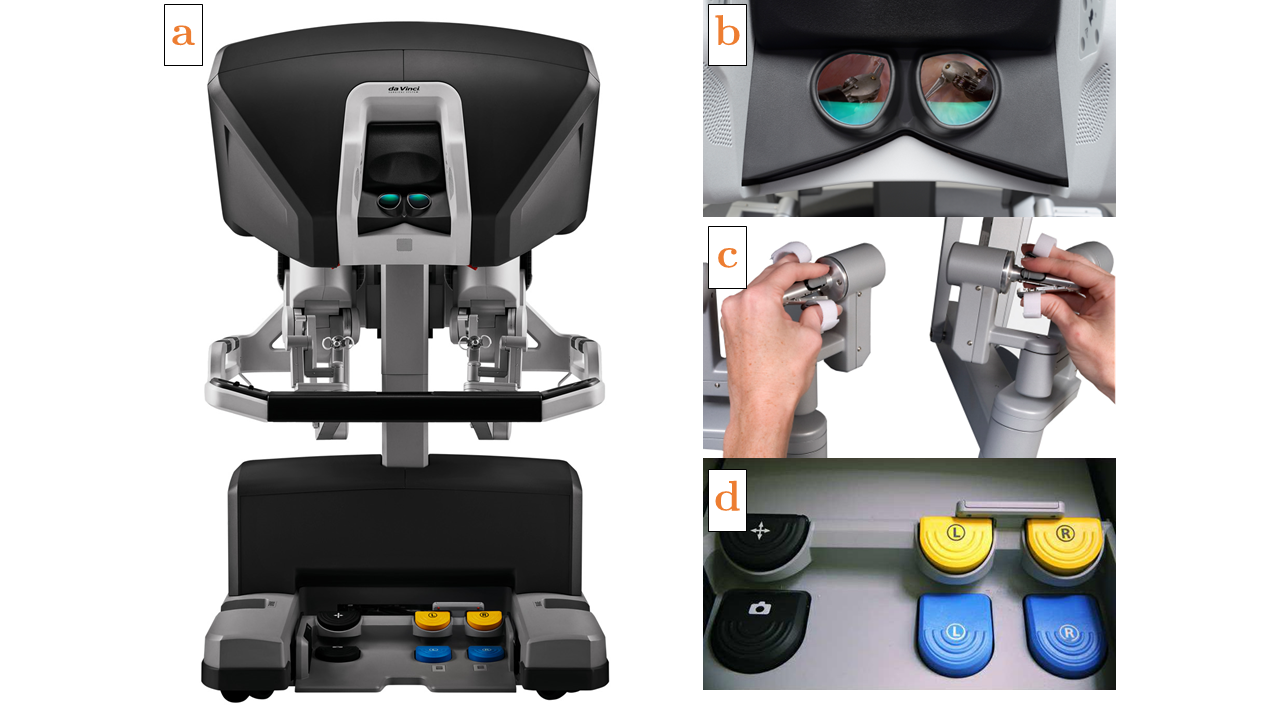
\includegraphics[width=\textwidth]{images/surgeon_cart_panel.png}
    \caption{a. The \davinci surgeon console; b. The \hrsv oculars; c. The \mtms; d. The foot switches}
    \label{fig:surgeonconsolepanel}
\end{figure}

\subsection{The Patient Cart}
A robot-assisted surgery with the \davinci is set up by positioning the patient cart in proximity of the surgical table: the relative position of the two depends on the type of operation to be executed. 
The cart is the frame of allocation for the \psms and the \ecm: the \ecm is the kinematic structure that controls the pose of the stereo endoscope camera, while the \psms are the robot arms that are used to position and rotate the surgical instruments. A standard \davinci robot mounts four \psms, controllable by two surgeons independently seated at two different consoles; however, a single surgeon can teleoperate a two-\psms-robot by himself as it's the case for this study.
The position of both \psms and the \ecm relative to the frame of the patient cart can be further adjusted to optimize their pose with respect to the surgical site and the type of operation to be performed: a set of 6 \acp{suj} can be used to position in space the base of each of the \psms and \ecm. The \ac{suj} kinematic chain consists of 1 prismatic joint and 5 revolute joints moved manually by the surgeon or the OR nurse during the pre-operative phase.


\paragraph{Patient-Side Manipulators} Each \psm is a 7-DOF actuated arm (5 revolute joints, 1 prismatic joint, and the gripper angle of opening), which moves a surgical instrument about a Remote Center of Motion (RCM), \textit{i.e.} a fixed fulcrum point that is invariant to the configuration of the PSM joints and the position of which is dependent only on the base link reference frame of the arm. When the surgeon or the \ac{or} nurse manually positions the \acp{suj}, ultimately he is positioning the RCM in space: because the RCM is a fixed fulcrum point, its position will not change while the \psm is moving. This feature is what makes the \davinci a truly minimally invasive technology, since if the RCM is positioned exactly at the surgical incision on the patient's body, the surgeon has a wide range of motion that will still not require a larger opening on the patient's skin. 

\begin{figure}[h!]
    \centering
    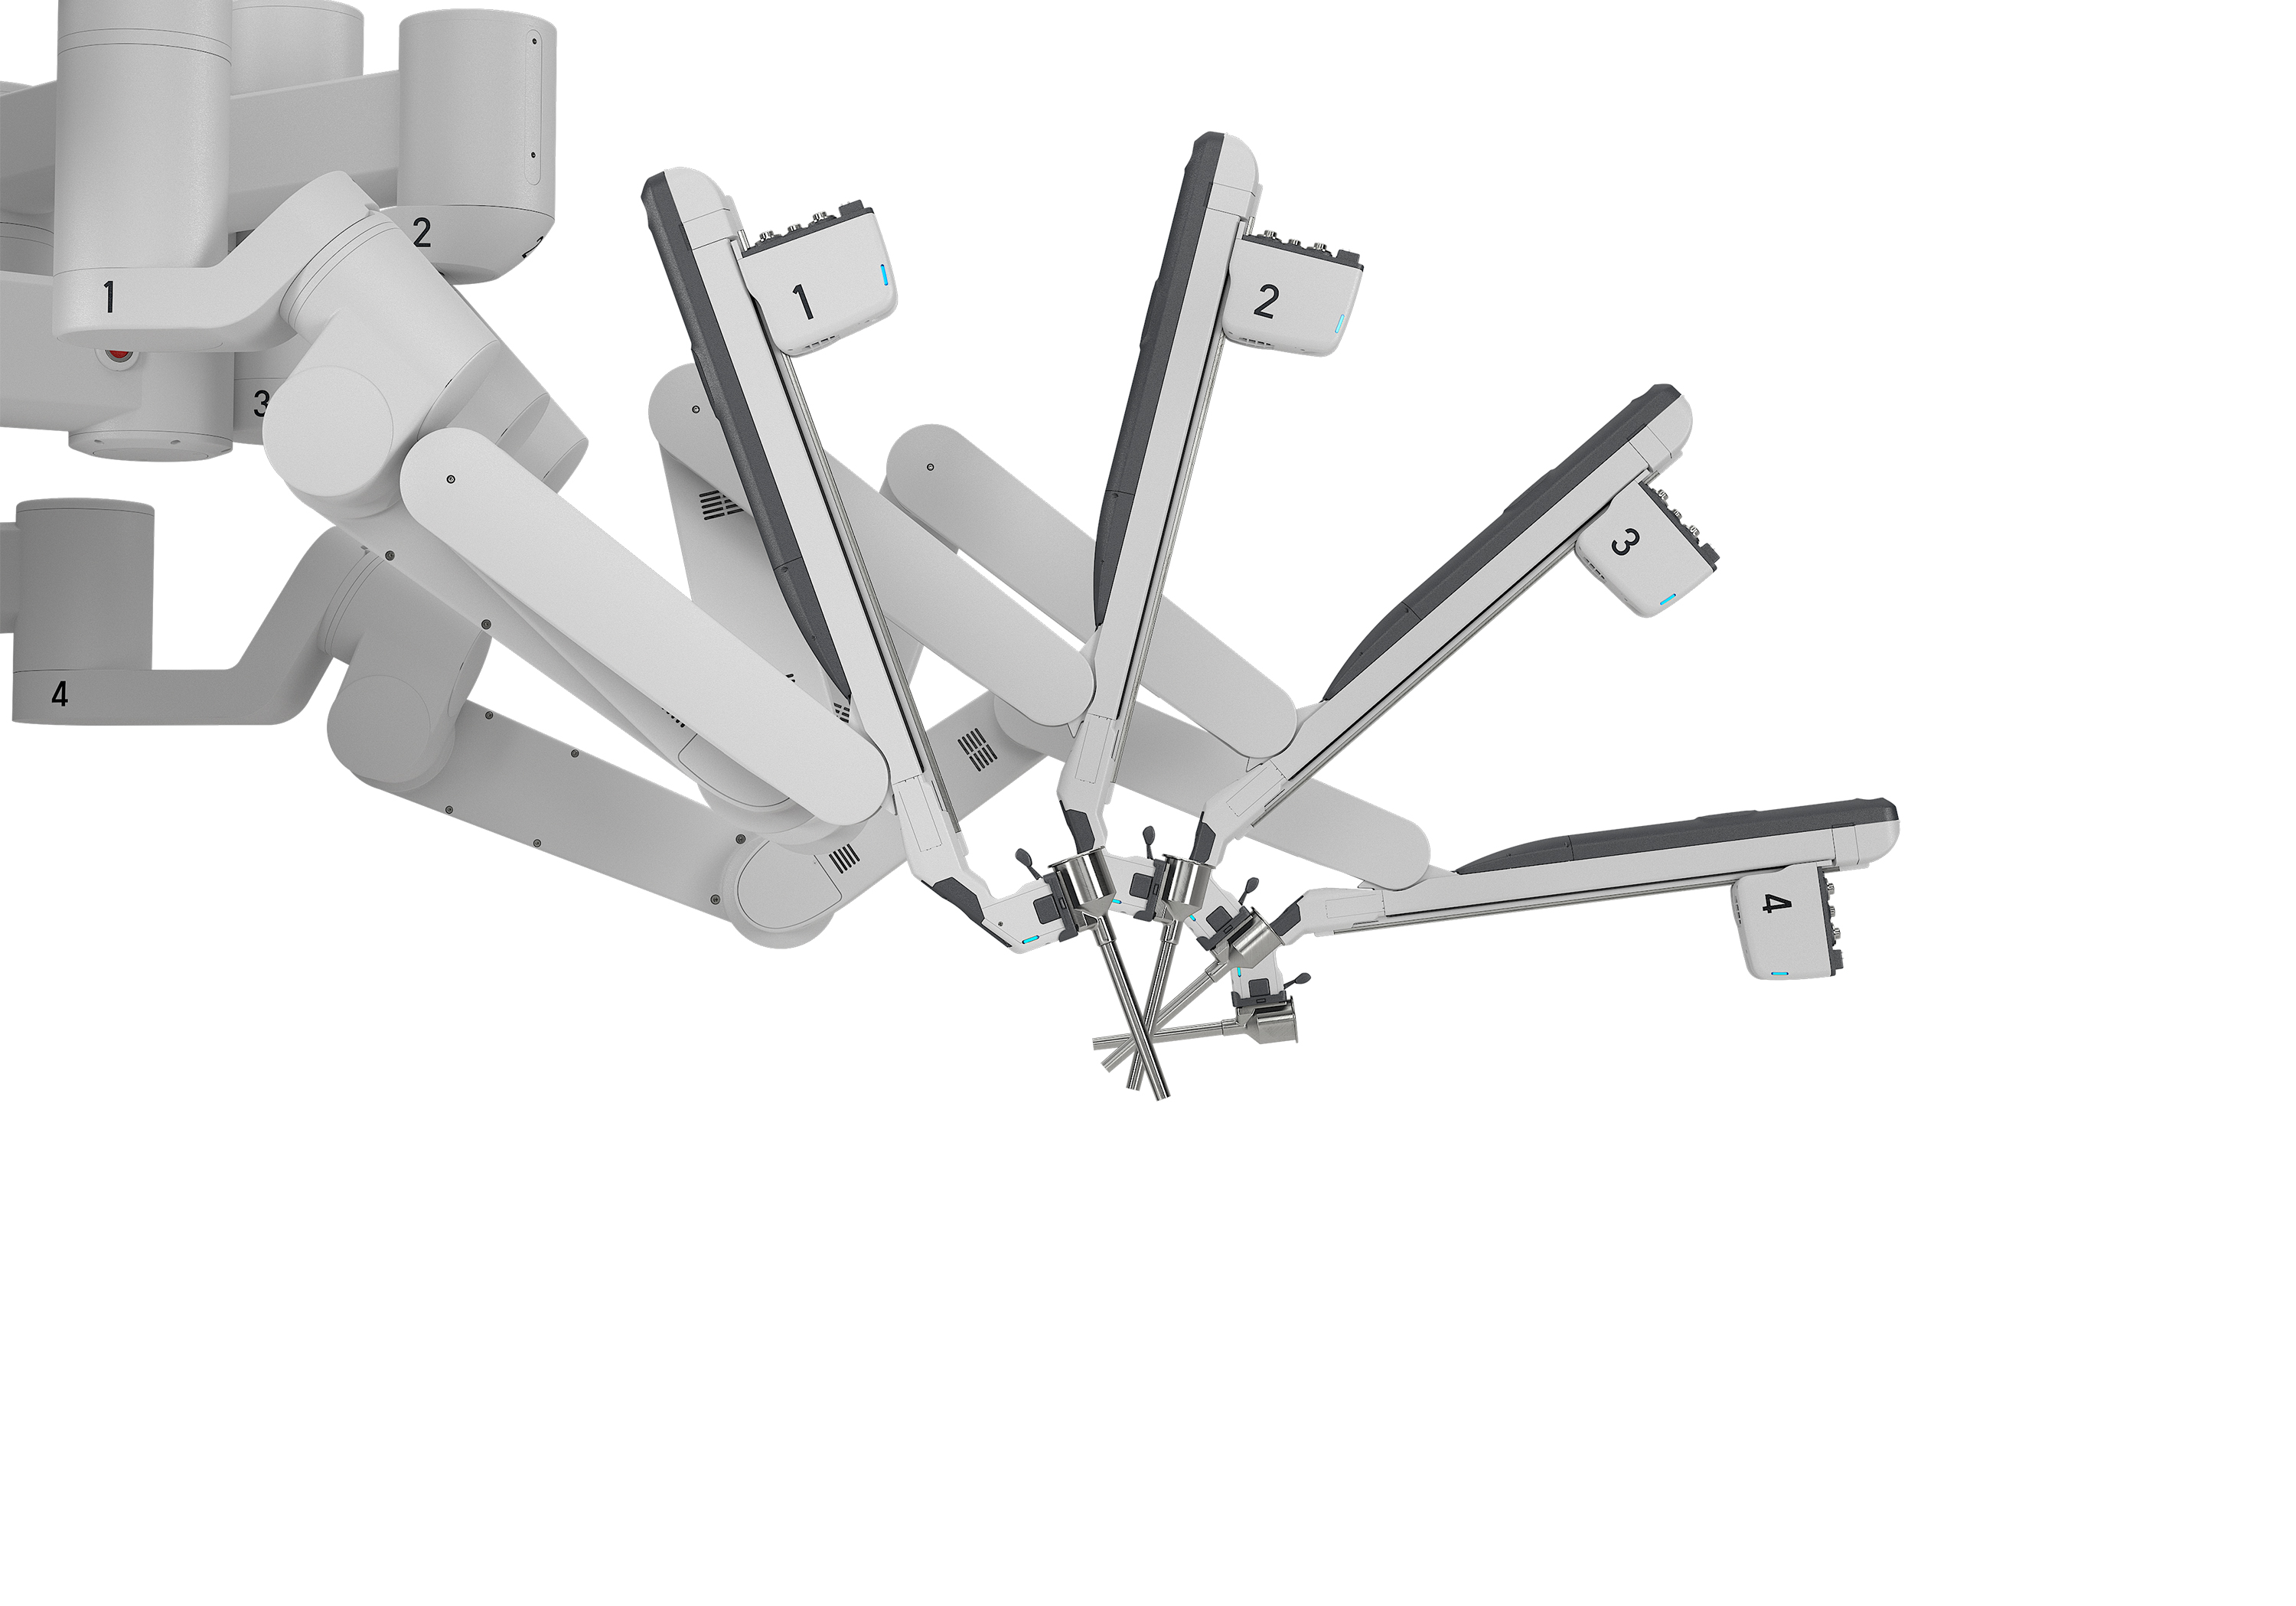
\includegraphics[width=0.5\textwidth]{images/rcm.jpg}
    \caption{A visual representation of the concept of Remote Center of Motion (RCM). Indepenently by the configuartion of the \psm, the RCM is always located at the same point in space.}
    \label{fig:rcm}
\end{figure}

Intuitive Surgical Inc. makes available a variety of surgical instruments that can be mounted on the \psms and that cover a vast range of use cases, from tissue manipulation to suturing to cauterization. An attachment mechanism unique for all instruments allows one to quickly swap them even during the procedure.

Each of the available instruments designed by Intuitive Surgical exploits the \textit{EndoWrist}\cright\xspace technology: a set of minuscule pulleys and cable allows the instruments' tooltips to achieve greater dexterity and range-of-motion when compared to the human wrist. This factor highly contributes to the minimally invasive nature of this surgical robot, as it permits achieving articulate and complex orientations that would require a larger incision if performed with a conventional approach.

\paragraph{Endoscope Camera Manipulator} One of the robotic arms mounted on the patient cart holds the stereo endoscope camera and determines its pose in space. Naturally, the position and orientation of the endoscope camera determine how the surgical scene is framed and, ultimately, what the surgeon sees in the \hrsv. Contrary to a standard laparoscopic approach where the endoscope placement is a responsibility of the assistant surgeon, with a \davinci robot it's the operating surgeon himself that controls the position of the camera. As a matter of fact, when the operator at the console desires to change the viewing point of the surgical scene, he switches the control from the \psms to the \ecm by pressing one of the foot pedals. While that pedal is held down, the control signal from the \mtms is sent to the \ecm instead of the \psms, which moves accordingly.

\begin{figure}[h]
    \centering
    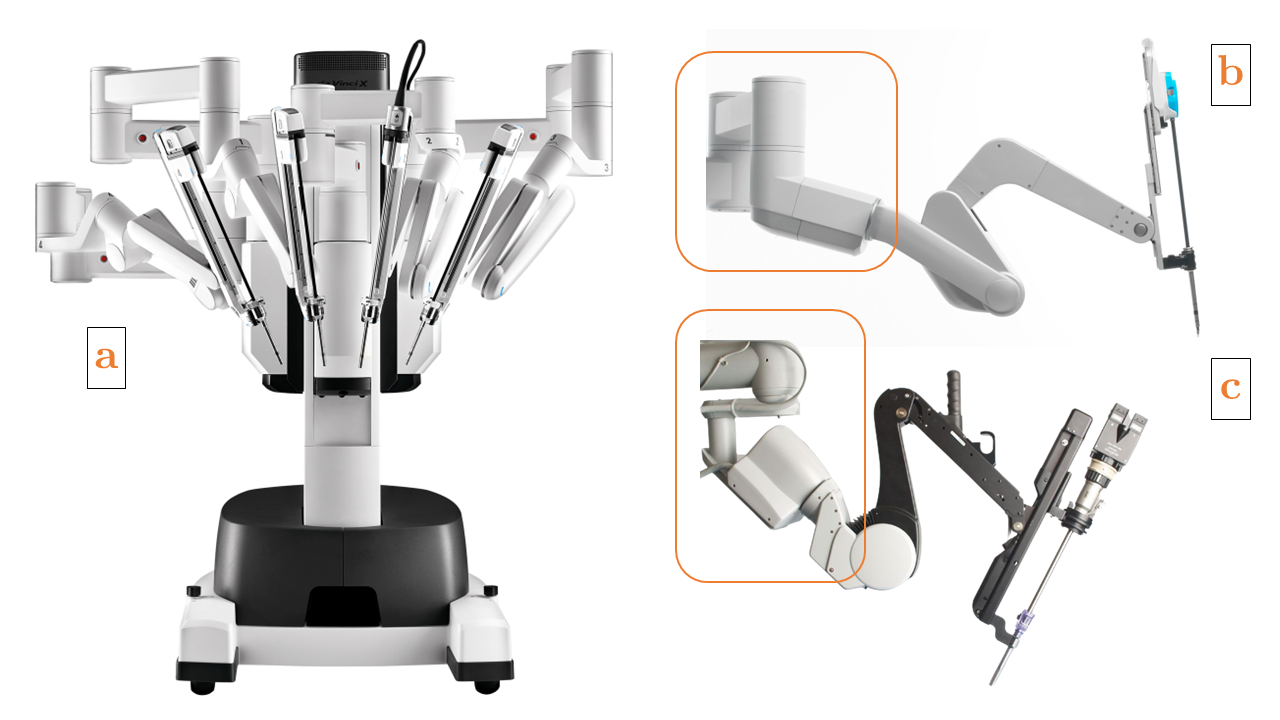
\includegraphics[width=\textwidth]{images/patient_cart_panel.png}
    \caption{a. The patient cart of the \davinci robot; b. A \psm; c. The \ecm; The \acp{suj} of the \psm and \ecm are in the orange boxes}
    \label{fig:patientcartpanel}
\end{figure}

\subsection{The Vision Cart} 
The computational, control and communication hardware is hosted on the vision cart, which acts as the main interface between the components. It is also responsible for computing FK and IK and for powering the motors, sensors and endoscope camera.

\section{VR Surgical Simulators}
Aghazadeh \textit{et al.} \cite{Aghazadeh2016} demonstrated a statistical correlation between robotic performance in a simulated environment and robotic clinical performance, effectively showcasing the potential of VR simulators for surgical training and their comparability to the standard dry-lab phantom training. Most of the surgical robotics companies on the market have developed and marketed their own general-purpose VR simulator, and a lot of research projects have been conducted to develop simulators for specific robotic platforms or for testing specialized applications.

Intuitive Surgical commercializes the \textit{daVinci SimNow} virtual surgical simulator  (previously \textit{dVSS, daVinci Skill Simulator}) as a skill-building framework for learning how to safely and successfully operate its surgical robot. It offers a realistic simulated environment comprising 47 skill exercises and 33 virtual surgical procedures, with performance tracking and procedure-specific feedback. 

Other relevant simulators on the market \cite{Bric2016} \cite{Kumar2015} are the \textit{Mimic dV-Trainer} (dV-Trainer; Mimic Technologies, Inc, Seattle, WA, USA), the \textit{Robotic Surgical Simulator} (RoSS; Simulated Surgical Systems, Buffalo, NY, USA), the \textit{Sim-Surgery Educational Platform} (SEP, SimSurgery, Norway), and the \textit{ProMIS} hybrid simulator (\textit{Canadian Aviation Electronics Healthcare, Canada}). 

In terms of augmenting the surgical tranining, visual assistance algorithms are present in most of the listed simulators, but haptic guidance is missing in all cases.

An anticipation of the role of virtual reality environments in surgery was published in the literature as early as 2001 \cite{McCloy2001}, while the very first research work on the topic developing and validating a \vr simulator interfaceable with the \davinci appeared in 2008 \cite{{Lendvay2008}}. From there, several studies and advancements have been published in literature \cite{Moglia2016}: initially, most of the work was focused on validating and comparing the simulators on the market, assessing their role in the acquisition of surgical skills in general \cite{Lerner2010} or for specific surgical fields \cite{Korets2011}. Later, the focus shifted towards the development of new simulators and the improvement of existing ones, with the goal of making them more realistic, effective and affordable \cite{Hardon2022}. 

In 2014 Smith \textit{et al.} established and summarized, upon a 14-society consensus, a set of basic robotic surgery skills that every training curriculum should include \cite{Smith2014}. 
The authors also proposed a set of guidelines for the development of a robotic surgical training curriculum, which is still valid today. This skillset is featuring pre, intra and post operatory skills: \ac{vr} simulators only cover intraoperative skills, but do so in quite a comprehensive and adaptive way. Surgical simulators can be, indeed, built and developed to train the surgeon in intensively improving a single one of such skills, or to train him in a more general way, covering all of them. Most of the \vr simulators developed in literature belong to the former category, and so do the assistive algorithms that they feature.

\section{Virtual Fixtures and Augmented Training}
The very first example of a \vf algorithm was implemented on a PUMA 560 robot and consisted of a real-time collision avoidance algorithm \cite{Khatib1986}. Since then, the concept of \vf has been extended to a wide range of robotic applications, including surgical robotics. 

The first definition of Virtual Fixtures was proposed by Louis B. Rosenberg, who proposed the concept of ``abstract sensory information overlaid on top of reflected sensory feedback from a remote environment'' \cite{Rosenberg1993}. More recently, Bowyer \textit{et al.} \cite{Bowyer2014} provided an extensive review that included most of the existing \vf algorithms and proposed a taxonomy of the different approaches. Neither \cite{Rosenberg1993} nor \cite{Bowyer2014}, however, analyzed the context of surgical robotics or the role of \vf in the training of surgeons, but rather circumstanced the topic in the broader field of \textit{telemanipulation}. 

One of the earliest research work indagating the role of \vfs for surgical training application concluded that the introduction of haptic guidance into a training protocol increases the reusability of paths generated with manual control \cite{Payandeh2002}. Similar positive results were obtained in the assessment of the benefits of a Guidance \textit{Trusted-Region} \vf in laparoscopic training \cite{Iranfar2018}, which was confirmed to improve the training process both in a real and in a simulated context. An Obstacle Avoidance (or Forbidden Region) Active Constraint was similarly shown to improve a training protocol conducted on a surgical simulator \cite{Hong2016}.

Clinically supported training curricula for surgical robotics are a crucial step in the global standardization of training and certification of surgeons for surgical robotics procedures \cite{Fisher2015}: many of them are in the early development stage and are still in the process of being validated. The role that haptic assistance could have in such curricula is still to be explored on a large scale, but the early research results are promising \cite{Van2009}.

% BIBLIOGRAPHY
% \bibliographystyle{unsrt}
% \bibliography{refs.bib}

\end{document}